\section{Introduction}
\begin{frame}{}
    \LARGE Reinforcement Learning: \textbf{Introduction}
\end{frame}

\begin{frame}[allowframebreaks]{RL - ICLR 2023}
    \begin{figure}
        \centering
        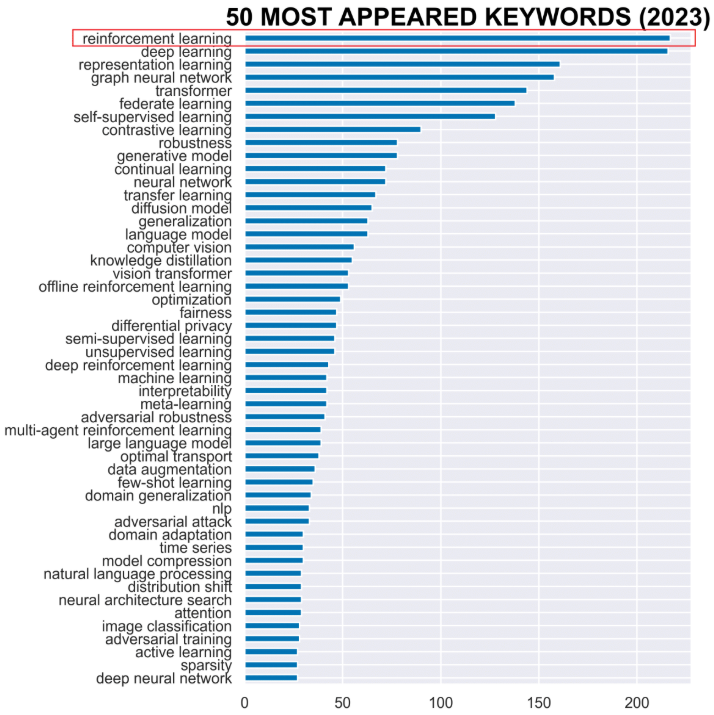
\includegraphics[height=0.8\textheight,width=\textwidth,keepaspectratio]{images/intro/most-popular.png}
        \caption*{Source: \href{https://github.com/EdisonLeeeee/ICLR2023-OpenReviewData}{ICLR 2023 - Open Review Data}}
    \end{figure}
\end{frame}

\begin{frame}[allowframebreaks]{Introduction}
    \textbf{Definition:} RL is a type of machine learning where agents learn to make decisions by interacting with an environment.

\framebreak
    {
        \large
        \textbf{Core Elements:}
        \begin{itemize}
            \item<1-> \textbf{Agent}: The learner or decision maker.
            \item \textbf{Environment}: The external system the agent interacts with.
            \item \textbf{State}: A representation of the current situation.
            \item \textbf{Action}: Choices the agent can make.
            \item \textbf{Reward}: Feedback signal for evaluating actions.
        \end{itemize}
    }
\framebreak
    \begin{figure}
        \centering
        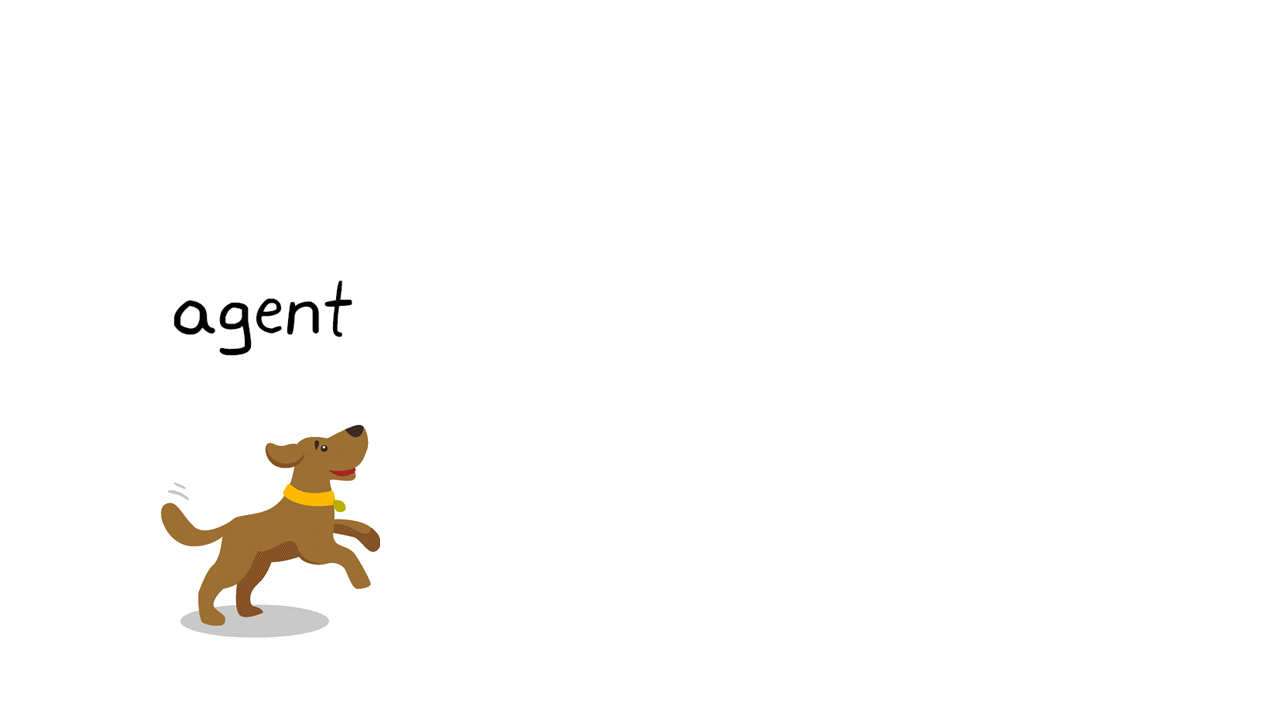
\includegraphics[height=0.9\textheight,width=\textwidth,keepaspectratio]{images/intro/agent.png}
    \end{figure}
\framebreak
    \begin{figure}
        \centering
        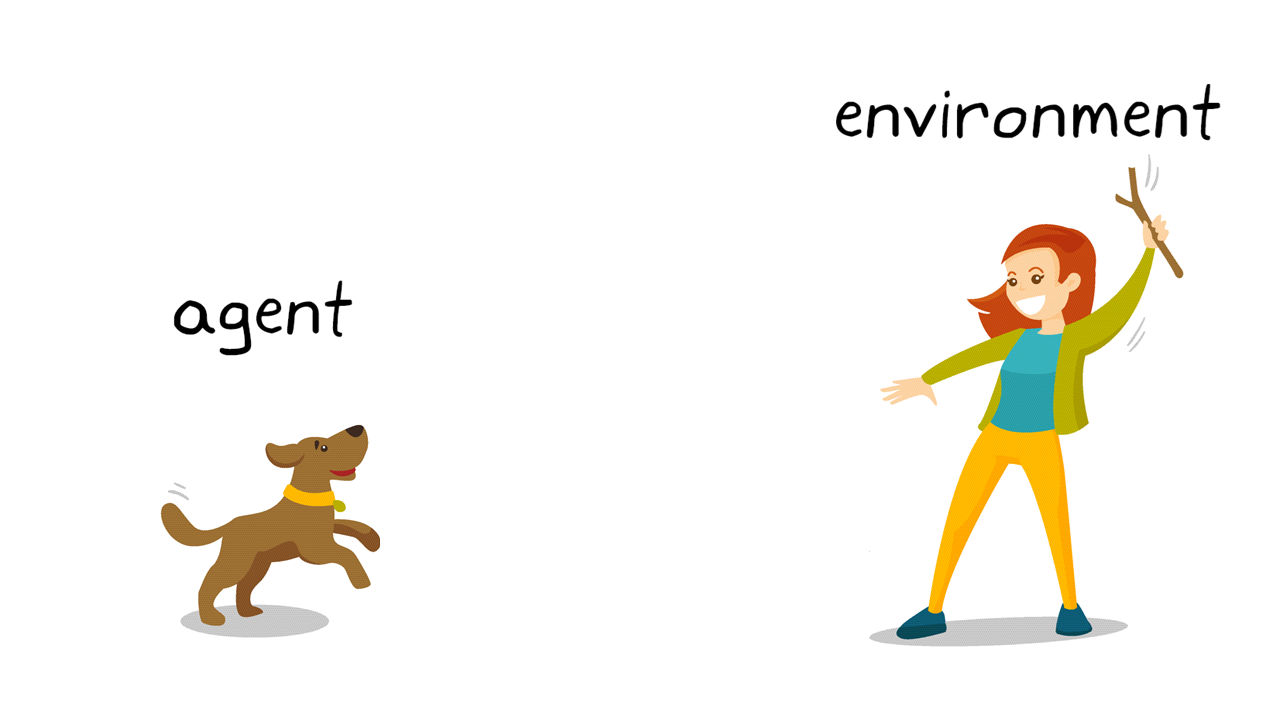
\includegraphics[height=0.9\textheight,width=\textwidth,keepaspectratio]{images/intro/enviroment.png}
    \end{figure}
\framebreak
    \begin{figure}
        \centering
        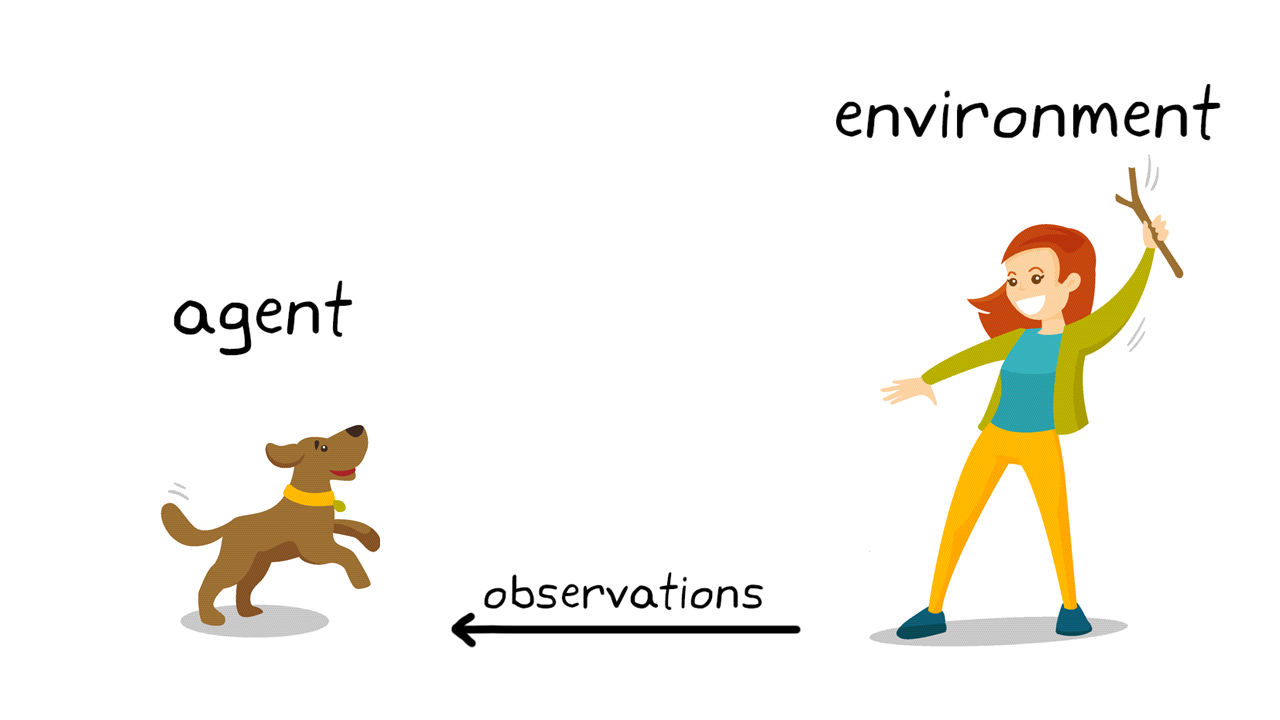
\includegraphics[height=0.9\textheight,width=\textwidth,keepaspectratio]{images/intro/observations.png}
    \end{figure}
\framebreak
    \begin{figure}
        \centering
        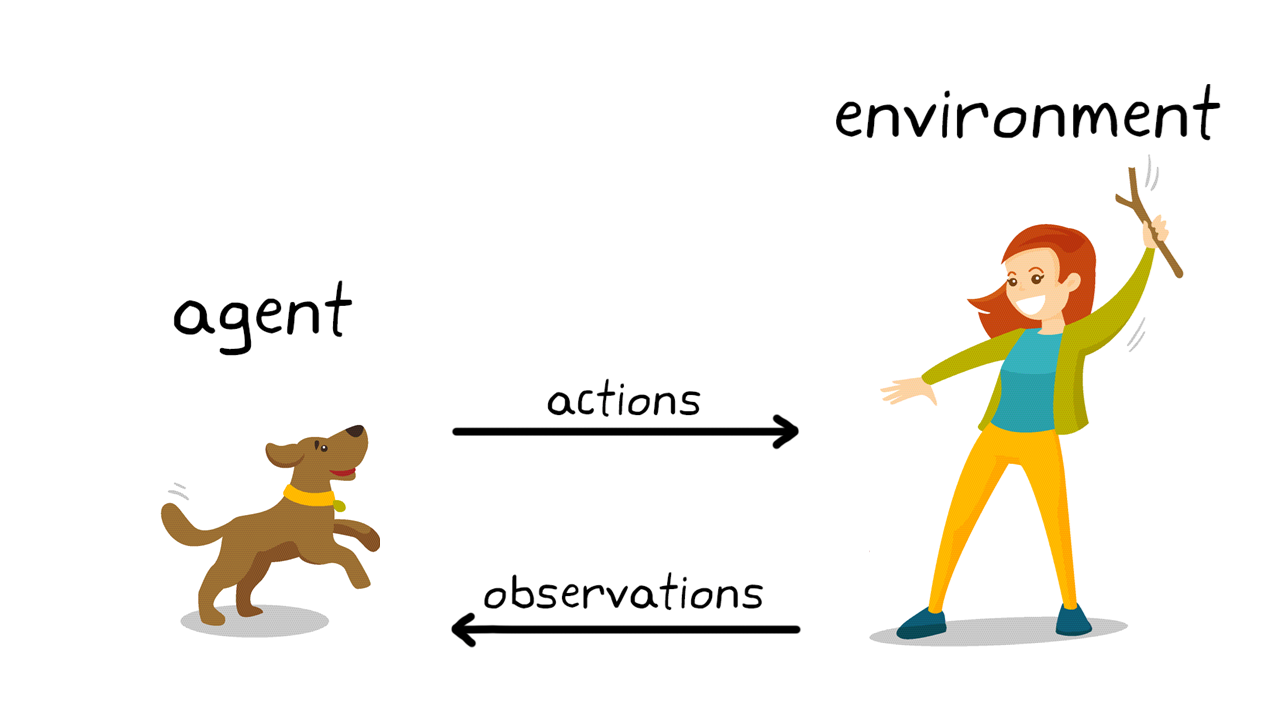
\includegraphics[height=0.9\textheight,width=\textwidth,keepaspectratio]{images/intro/actions.png}
    \end{figure}
\framebreak
    \begin{figure}
        \centering
        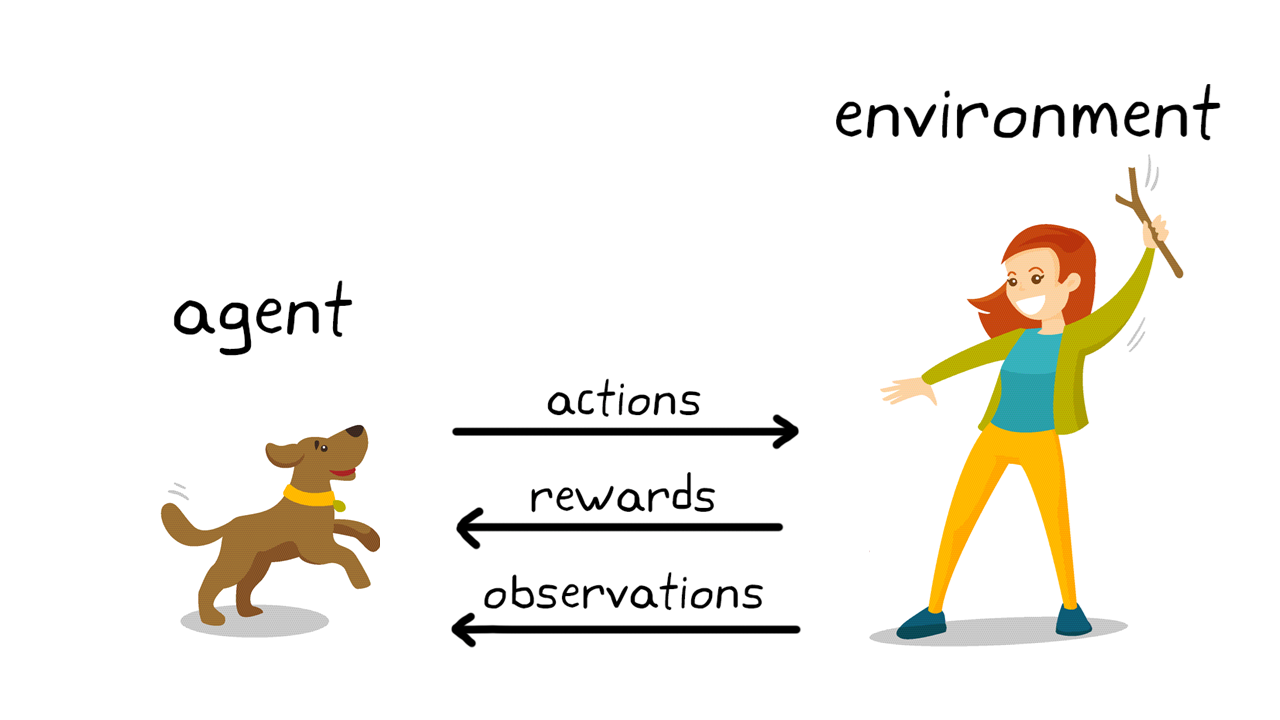
\includegraphics[height=0.9\textheight,width=\textwidth,keepaspectratio]{images/intro/rewards.png}
    \end{figure}
\framebreak
    {
        \large
        \textbf{Key Concepts:}
        \begin{itemize}
                \item Agent interacts with environment.
                \item Learns by trial and error.
        \end{itemize}
    }

\framebreak
    {
        \large 
        \textbf{How does it work?}
        \begin{itemize}
            \item Agent gets rewards or penalties.
            \item Goal: Maximize cumulative reward (a.k.a. return).
        \end{itemize}
    }
\end{frame}

\begin{frame}[allowframebreaks]{}
    \foreach \i in {11,...,23} { % Integers from 1 to 5
        \begin{figure}
            \centering
            \includegraphics[height=0.9\textheight,width=1\textwidth,keepaspectratio]{images/intro/step-\i.png}
        \end{figure}

        \framebreak
    }
\end{frame}

\begin{frame}{Supervised Learning vs. Reinforcement Learning}
    \begin{columns}[T]
        \column{0.5\textwidth}
            \textbf{Supervised Learning}
            \begin{itemize}
                \setlength{\itemsep}{1.5em}
                \item Given labeled data: $\{(x_i, y_i)\}$, learn $f(x) \approx y$
                \item Directly told what to output
                \item Inputs $x$ are independently, identically distributed (i.i.d.)
            \end{itemize}
        \column{0.5\textwidth}
            \textbf{Reinforcement Learning}
            \begin{itemize}
                \setlength{\itemsep}{1.5em}
                \item Learn behavior $\pi(a|s)$
                \item Learn from experience, indirect feedback
                \item Data not i.i.d.: actions affect future observations
            \end{itemize}
    \end{columns}
\end{frame}

\begin{frame}[allowframebreaks]{Examples of Reinforcement Learning}
    % Define arrays of headings and footers
    \newcommand{\exampleheading}[1]{%
        \ifcase#1
            \or ChatGPT%
            \or Healthcare%
            \or Multiagent Hide \& Seek%
            \or Multiagent Hide \& Seek%
            \or Gran Turismo GTSophie%
            \or Autonomous Driving%
            \or AlphaGo%
            \or Muzero%
            \or Minecraft%
            \or More Examples%
        \fi
    }
    \newcommand{\examplefooter}[1]{%
        \ifcase#1
            \or \href{https://openai.com/blog/chatgpt}{https://openai.com/blog/chatgpt}%
            \or \href{https://dl.acm.org/doi/abs/10.1145/3477600}{Yu, et al. Reinforcement Learning in Healthcare: A Survey}%
            \or %
            \or %
            \or \href{https://www.gran-turismo.com/us/gran-turismo-sophy/technology/}{https://www.gran-turismo.com/us/gran-turismo-sophy/technology/}%
            \or \href{https://ieeexplore.ieee.org/abstract/document/9351818}{Kiran, et al. Deep Reinforcement Learning for Autonomous Driving: A Survey}%
            \or \href{https://www.tomshardware.com/news/alphago-narrow-win-ke-jie,34486.html}{https://www.tomshardware.com/news/alphago-narrow-win-ke-jie,34486.html}%
            \or \href{https://www.deepmind.com/blog/muzero-mastering-go-chess-shogi-and-atari-without-rules}{https://www.deepmind.com/blog/muzero-mastering-go-chess-shogi-and-atari-without-rules}%
            \or \href{https://www.artificialintelligence-news.com/2022/06/29/ai-learns-how-to-play-minecraft-by-watching-videos/}{https://www.artificialintelligence-news.com/2022/06/29/ai-learns-how-to-play-minecraft-by-watching-videos/}%
            \or \href{https://phys.org/tags/reinforcement+learning/}{https://phys.org/tags/reinforcement+learning/}%
        \fi
    }

    \foreach \i in {1,...,10} {
        \begin{figure}
            \centering
            {\large \exampleheading{\i}} \\
            \includegraphics[height=0.7\textheight,width=1\textwidth,keepaspectratio]{images/intro/example-\i.png}\\
            \vspace{1em}
            {\small \examplefooter{\i}}
        \end{figure}
        \framebreak
    }
\end{frame}

